Es la dispersión de la luz visible o cualquier otra radiación electromagnética por partículas cuyo tamaño es mucho menor que la longitud de onda de los fotones dispersados. Ocurre cuando la luz viaja por sólidos y fluidos transparentes, pero se ve con mayor frecuencia en los gases. La dispersión de la luz solar en la atmósfera es la principal razón de la coloración del cielo.

\begin{figure}[H]
  \centering
  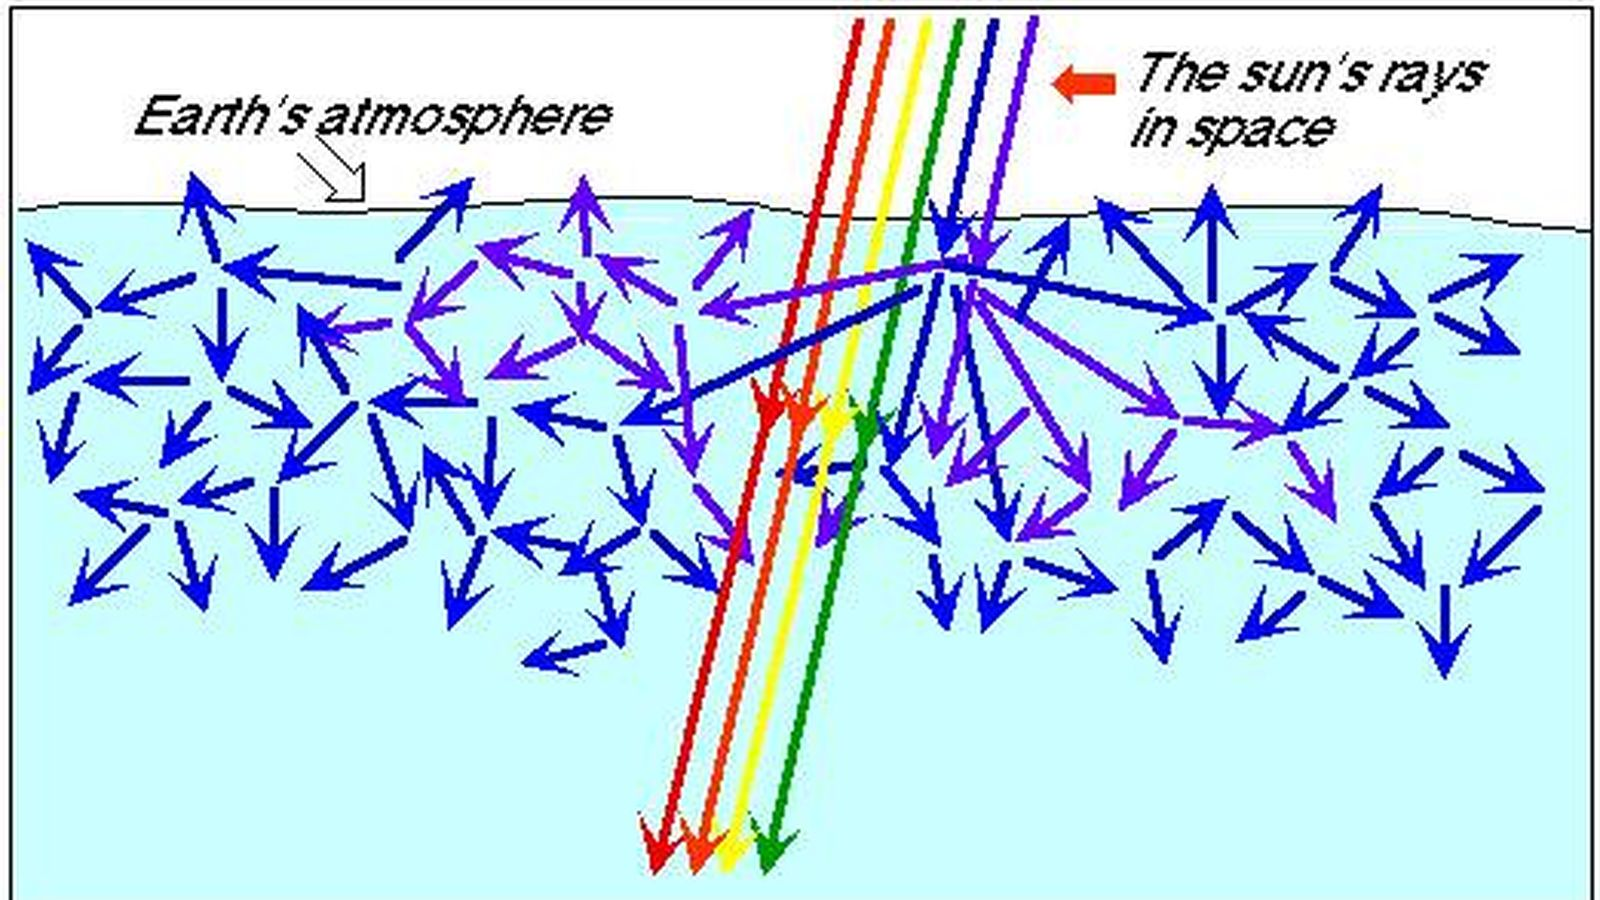
\includegraphics[scale=0.2]{imagenes/rayleigh.png}
  \caption{Dispersión de Rayleigh\cite{confrayleigh}}
\end{figure}

Al encontrar poca resistencia, como en el medio día, los rayos azules se dispersan en la atmósfera. Al encontrar mucha resistencia, como el amanecer o atardecer, los rayos rojos y anaranjados se dispersan.
